\documentclass[11pt]{article}
\usepackage{amsmath}
\usepackage[margin=.75in]{geometry}
\usepackage{enumitem}
\usepackage{float}
\usepackage{graphicx} % Required for inserting images
\usepackage{helvet}
\usepackage{hyperref}
\usepackage{listings}
\usepackage{mathptmx}
\usepackage{nameref}
\usepackage{pgfplots}
\usepackage{placeins}
\usepackage{subcaption}
\usepackage{titlesec}
\usepackage{wrapfig}
\renewcommand{\familydefault}{\sfdefault}
\graphicspath{{./images/}}

\titlespacing*{\section}{0pt}{0.2\baselineskip}{0.2\baselineskip}
\titlespacing*{\subsection}{0pt}{0.25\baselineskip}{0.25\baselineskip}
\titlespacing*{\subsubsection}{0pt}{0.1\baselineskip}{0.1\baselineskip}

\title{Complex Systems and Networks HW 2}
\author{Rachael Judy, Connor Klein, Josh Smith}
\date{31 March 2024}

\begin{document}
	\pgfplotsset{compat=1.18}
	\setlist[itemize]{noitemsep}
	\setlist[enumerate]{noitemsep}
	
	\maketitle
\section{Section 1: Random Policies and Social Recommendation Policy}\label{sec:q1}
\subsection{Simulation Description}\label{subsec:simulation}
% discuss hyperparameters like trials, epochs
This simulation uses variations on the Schelling model exploring Red and Green agents occupying a percentage of a 2-dimensional LxL grid. The agents prefer to be near their own type and are fully happy if at k or more of the eight neighbors are of the same type. The simulation is designed with hyperparameters of a 40x40 (L=40) square grid with wraparound at the borders. The agents occupy 90\% ($\alpha=.9$) of the cells and k=3 neighbors define the requirementn for total happiness of the agent. The number of trials run for each case is set to 20 trials of 20 epochs. Each epoch consists of moving every agent in the automata in a random order if the agent is unhappy. Different relocation policies and their parameters are applied to determine where unhappy agents move to seek greater satisfaction.

\subsubsection{Happiness Function}
An agent is defined as completely happy if k or more of its neighbors are of the same group as itself. The agent will have partial happiness represented by a linear combination of the count of matching neighbors and empty plots nearby. This function will be $H(A_i) = \frac{\text{count}(N_i) + .125 \text{count}(N_e)}{8}$ where H is the happiness of an agent A of type i, $N_i$ is a neighbor of type i, and $N_e$ is an adjacent empty square.

\subsubsection{Performance Metric}
The performance metric was selected to simply be the sum of the happiness of every agent in the cellular automata ie $\sum\limits_{a \in A} H(a)$.

\subsection{Policies}\label{subsec:policies}
The agent will consider moving only if it is unhappy. The policies modeled as described in the homework description are a random move policy and a social network recommendation policy. The random move policy has a single parameter $q$ which limits how many random empty cells to visit looking for a cell where the agent will be happier than it is currently. 

The social network recommendation (SNR) will take a randomly selected set of n friends for each agent who will look in a pxp square around themselves and report suitable squares found. The agent than randomly selects one of the suitable squares and moves there. If none is available, it defaults to the random move policy. This policy is considered over parameter values of p=[3,5] and n=[5, 10, 20].

\subsection{Results}
% for insertion of before/after plots
	\begin{figure}[h]
		\centering
		\begin{subfigure}{0.14\textwidth}
			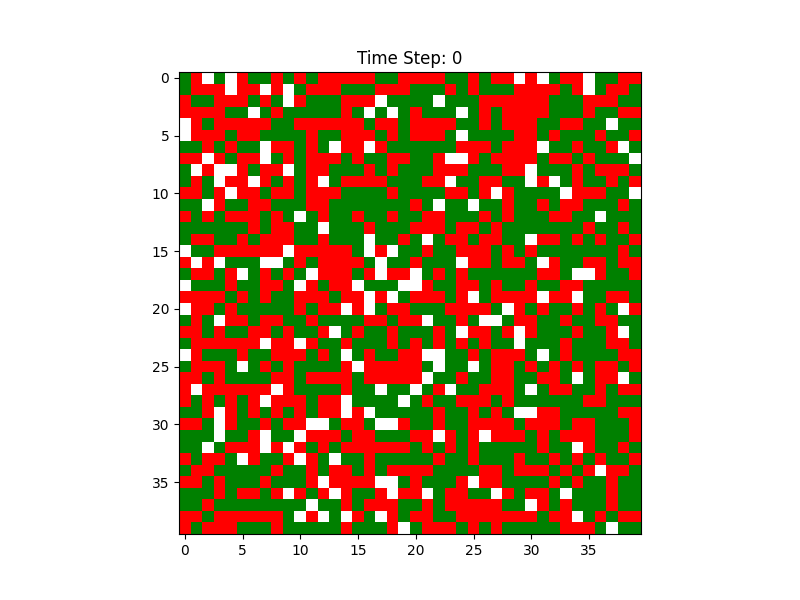
\includegraphics[width=\linewidth]{initial_random.png}
			\caption{\centering Random move}
		\end{subfigure}\hfill
		\begin{subfigure}{0.14\textwidth}
			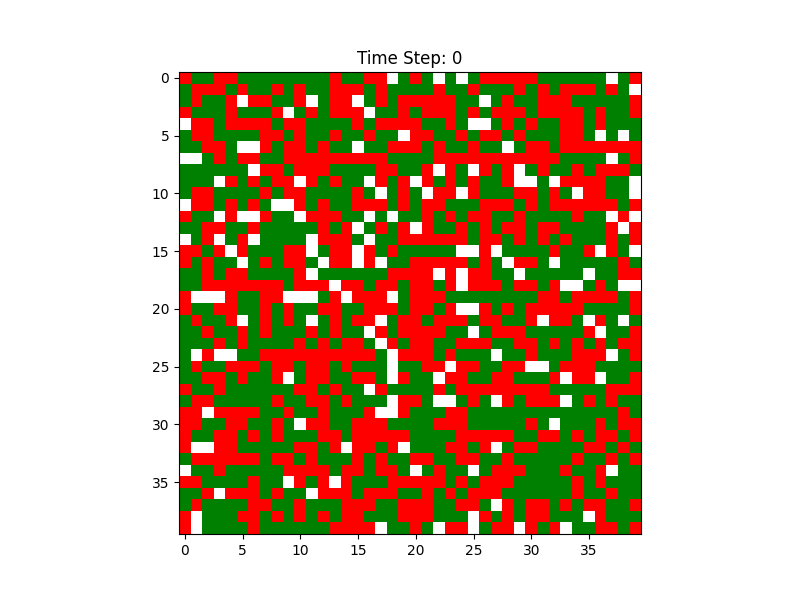
\includegraphics[width=\linewidth]{initial_social_n5p3.png}
			\caption{\centering SNR n=5, p=3}
		\end{subfigure}\hfill
		\begin{subfigure}{0.14\textwidth}
			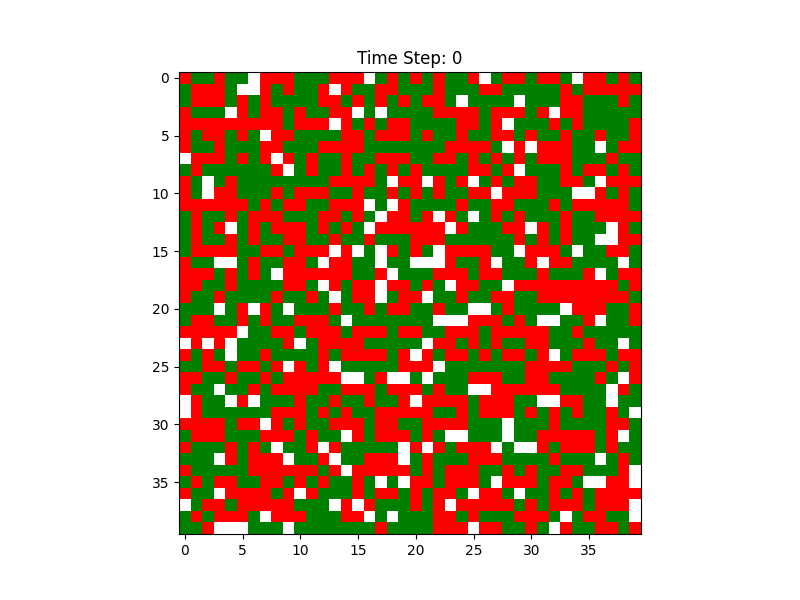
\includegraphics[width=\linewidth]{initial_social_n5p5.png}
			\caption{\centering SNR with n=5, p=5}
		\end{subfigure}\hfill
		\begin{subfigure}{0.14\textwidth}
			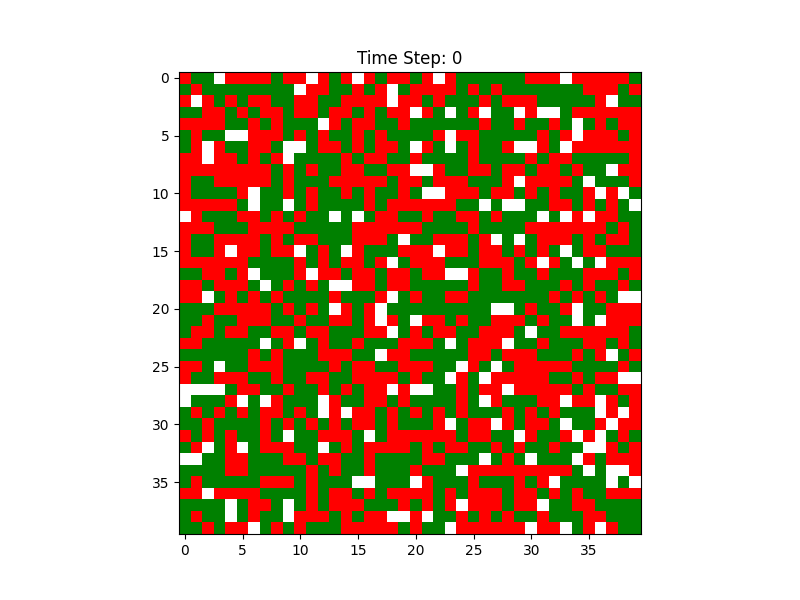
\includegraphics[width=\linewidth]{initial_social_n10p3.png}
			\caption{\centering SNR with n=10, p=3}
		\end{subfigure}\hfill
		\begin{subfigure}{0.14\textwidth}
			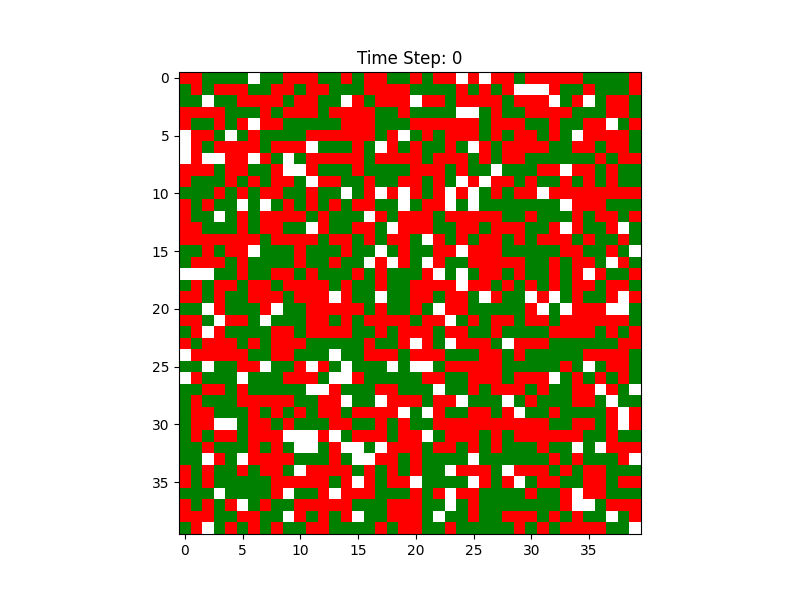
\includegraphics[width=\linewidth]{initial_social_n10p5.png}
			\caption{\centering SNR with n=10, p=5}
		\end{subfigure}\hfill
		\begin{subfigure}{0.14\textwidth}
			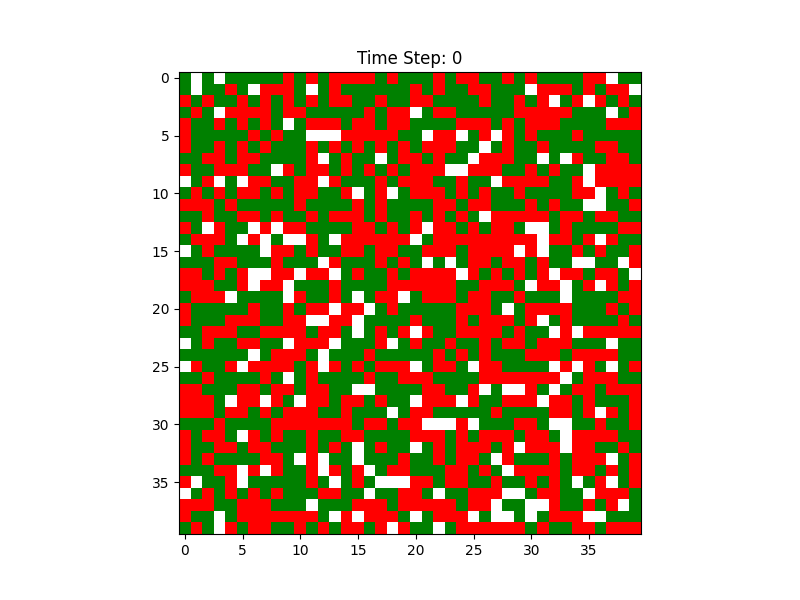
\includegraphics[width=\linewidth]{initial_social_n20p3.png}
			\caption{\centering SNR with n=20, p=3}
		\end{subfigure}\hfill
		\begin{subfigure}{0.14\textwidth}
			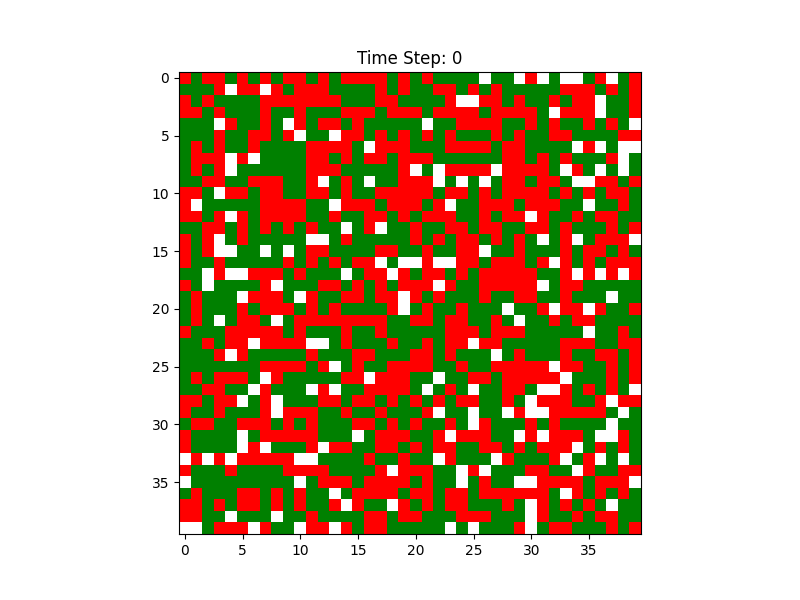
\includegraphics[width=\linewidth]{initial_social_n20p5.png}
			\caption{\centering SNR with n=20, p=5}
		\end{subfigure}
		\caption{Initial states for random move and social network recommendation policies}
	\end{figure}
	\vspace{-1em} % Adjust the vertical space here
	\begin{figure}[h]
		\centering
		\begin{subfigure}{0.14\textwidth}
			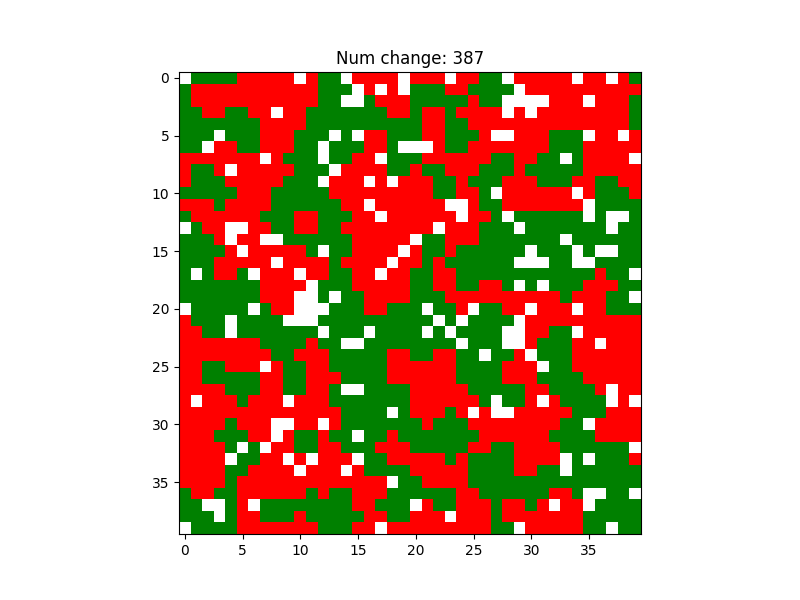
\includegraphics[width=\linewidth]{final_random.png}
			\caption{\centering Random move}
		\end{subfigure}\hfill
		\begin{subfigure}{0.14\textwidth}
			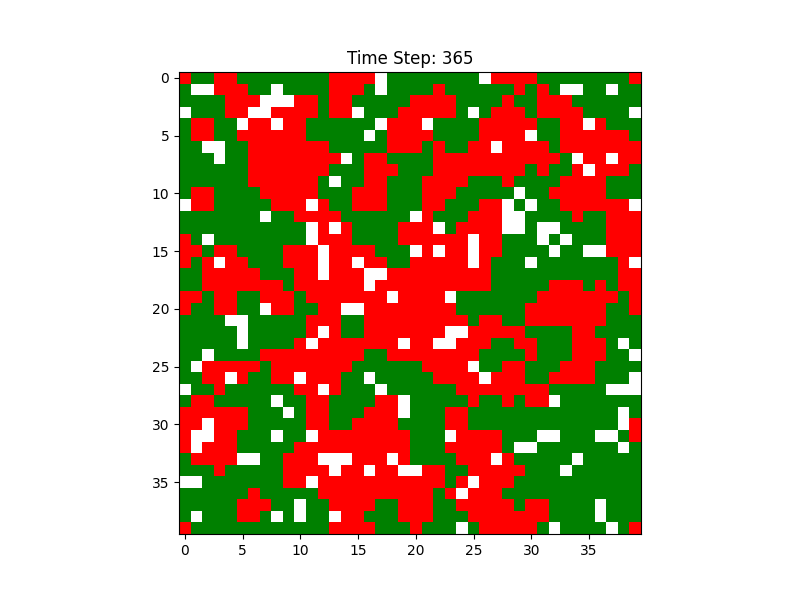
\includegraphics[width=\linewidth]{final_social_n5p3.png}
			\caption{\centering SNR with n=5, p=3}
			\label{n5p3}
		\end{subfigure}\hfill
		\begin{subfigure}{0.14\textwidth}
			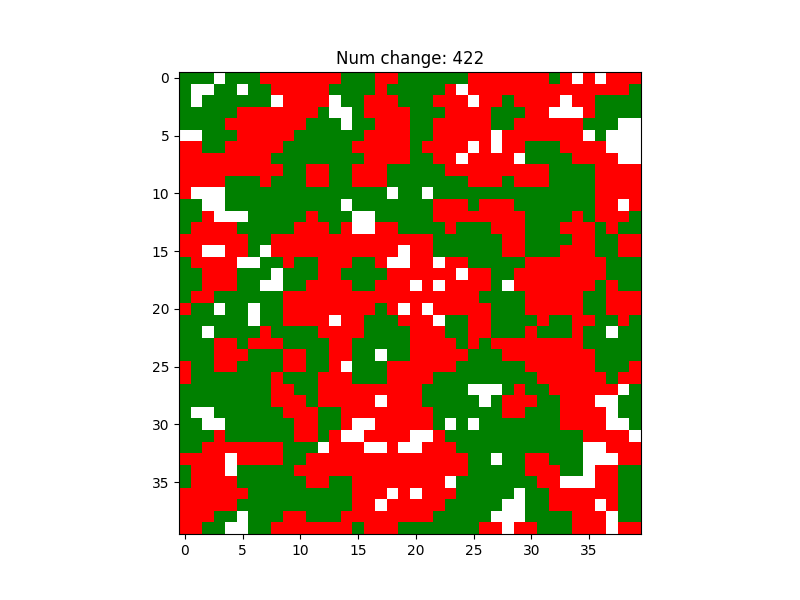
\includegraphics[width=\linewidth]{final_social_n5p5.png}
			\caption{\centering SNR with n=5, p=5}
		\end{subfigure}\hfill
		\begin{subfigure}{0.14\textwidth}
			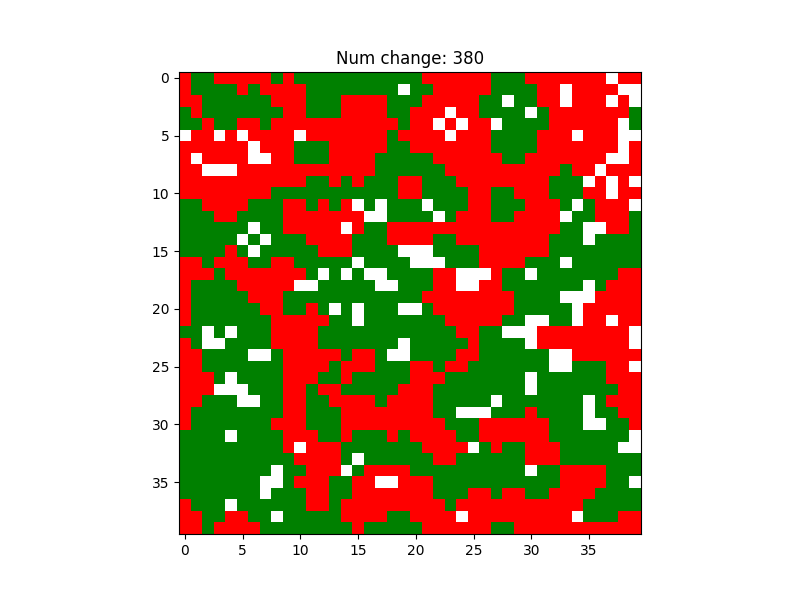
\includegraphics[width=\linewidth]{final_social_n10p3.png}
			\caption{\centering SNR with n=10, p=3}
		\end{subfigure}\hfill
		\begin{subfigure}{0.14\textwidth}
			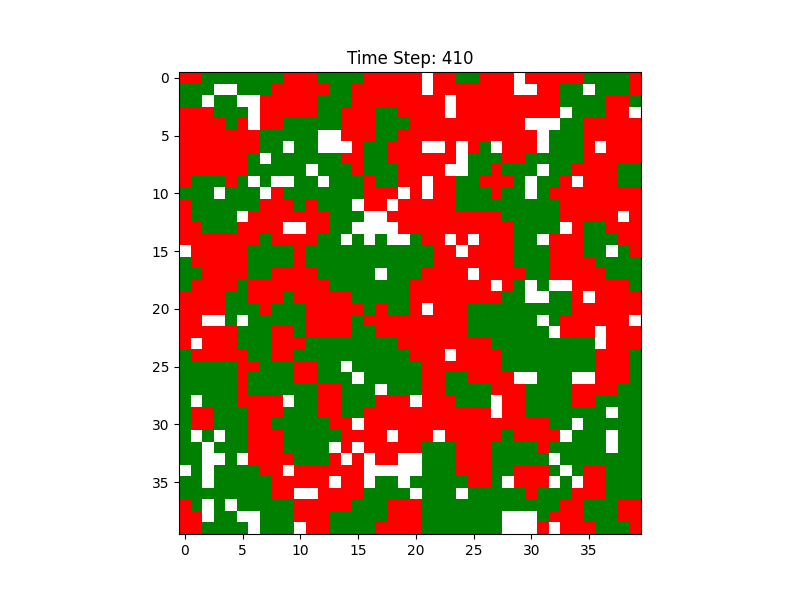
\includegraphics[width=\linewidth]{final_social_n10p5.png}
			\caption{\centering SNR with n=10, p=5}
		\end{subfigure}\hfill
		\begin{subfigure}{0.14\textwidth}
			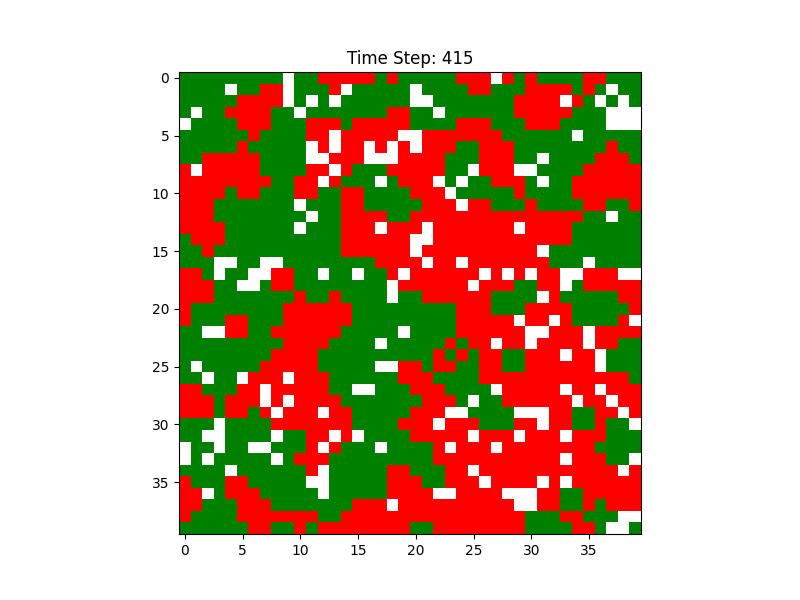
\includegraphics[width=\linewidth]{final_social_n20p3.png}
			\caption{\centering SNR with n=20, p=3}
		\end{subfigure}\hfill
		\begin{subfigure}{0.14\textwidth}
			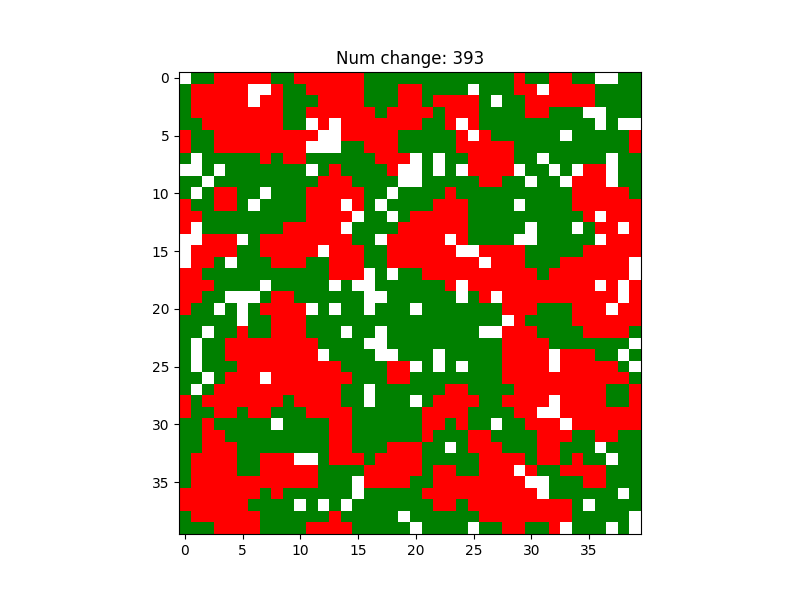
\includegraphics[width=\linewidth]{final_social_n20p5.png}
			\caption{\centering SNR with n=20, p=5}
		\end{subfigure}
		\caption{Final states of random move and social network recommendation policies}
	\end{figure}
	\vspace{-1em} % Adjust the vertical space here
	\begin{figure}[h]
		\centering
		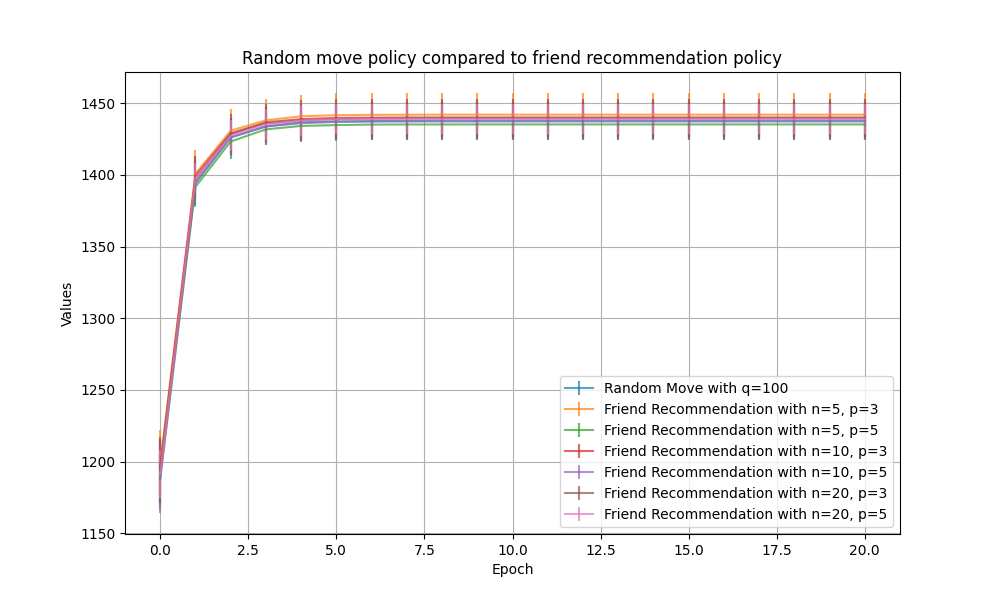
\includegraphics[width=\textwidth]{policies01.png}
		\caption{Time series comparing a random move policy with the social network recommendation policy}
		\label{p2_ts}
	\end{figure}
	\FloatBarrier
	All the experiments show that given a set number of epochs agents do tend to group up together. However, the size of the grouping seems to vary based on the number of friend recommendations and the area of those recommendations. As the number of friends making recommendations increased, the neighborhoods became smaller and more connected. Those with only five friends had more islands form as well. It was also shown that as the space of which the friends could recommend, or the value of \textit{p}, increased the connectiveness of the neighborhoods also increased. With both a high number of friends and a large area of recommendation search, the neighborhoods were well connected and spanned across the wrapped around board. The smaller values of \textit{n} and \textit{p}, resulted in smaller disconnected neighborhoods, usually in grouping of four. Four makes sense here as there was the minimum \textit{k} value in which an agent was set to be happy. It would be expected that smaller islands would form if \textit{k} was smaller as agents would opt out of moving. \par
	Fig \ref{p2_ts} describes that on average the setting that produced the happiest agents were those with a smaller group of friends to ask, who had a minimum knowledge of the area around them, see Fig \ref{n5p3}. However, the worst performing agents were those who had the same number of friends but those who had more knowledge of viable tiles, which is illustrated in Fig \ref{n5p5}. From there the happiness decreased with more friends and those friends knowing more spaces. If parallels could be drawn to real life from this simulation; it might suggest that having a few close friends may be more beneficial than many branching ones. \par
	However, even with the addition of a recommendation network, happiness appeared to converge around the same time, that is at around three epochs as shown on Fig \ref{p2_ts}. Also, the all the agents were significantly happier than in their starting states. This describes the mutually beneficial concept of taking turns in moving with all the agents able to decide if they would like to move with equal probability. If certain groups of agents were at a higher likelihood of choosing if they would like to move, this overall happiness might decrease. 
	


	\newpage
	\section{Section 2: Specialized Policies}
	\subsection{Rachael}
	\subsubsection{Policy Description}
	The segregation in housing application can be expanded to include searching within one's own neighborhood (SN) for a better house in the same area. The policy parameter $w$ defines the degree of separation from a neighbor, represented as the number of plots away from one's own plot the agent will travel to ask for recommendations and parameter $\beta$ defines the probability that a neighbor who is not the same type as the searcher is asked for available spots. This simulates asking neighbors of the same type in the area with a small chance of consulting neighbors of a different type. If none of the neighbors are aware of a good spot, the agent randomly moves. This policy is implemented as a BFS from the agent along matching agents up to the degree of separation limit.
	
	\subsubsection{Results}
	% for insertion of before/after plots
	\begin{figure}[h]
		\centering
		\begin{subfigure}{0.14\textwidth}
			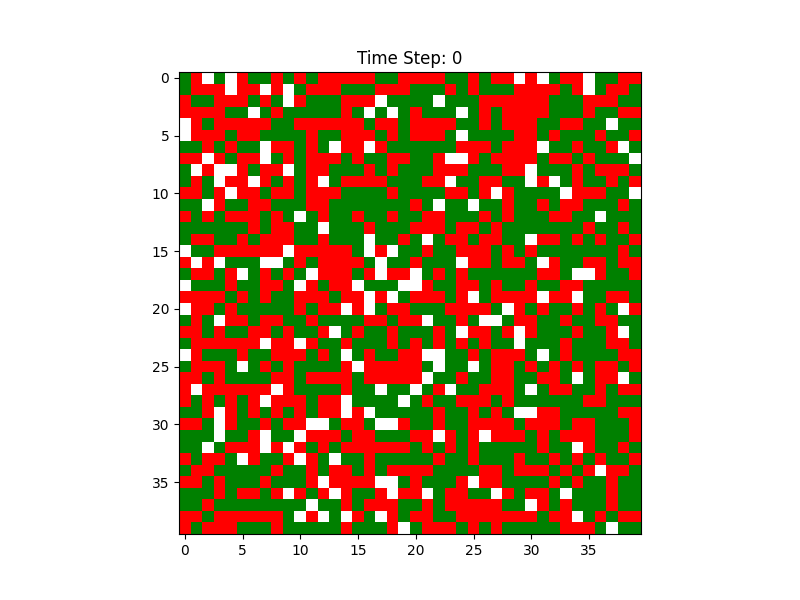
\includegraphics[width=\linewidth]{initial_random.png}
			\caption{\centering Random move}
		\end{subfigure}\hfill
		\begin{subfigure}{0.14\textwidth}
			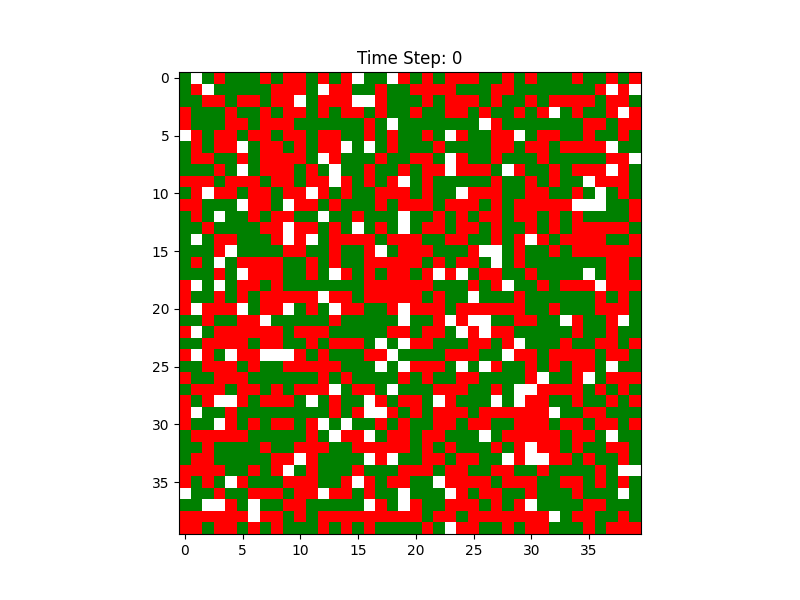
\includegraphics[width=\linewidth]{initial_cluster_w5b10.png}
			\caption{\centering SN w=5, beta=.1}
		\end{subfigure}\hfill
		\begin{subfigure}{0.14\textwidth}
			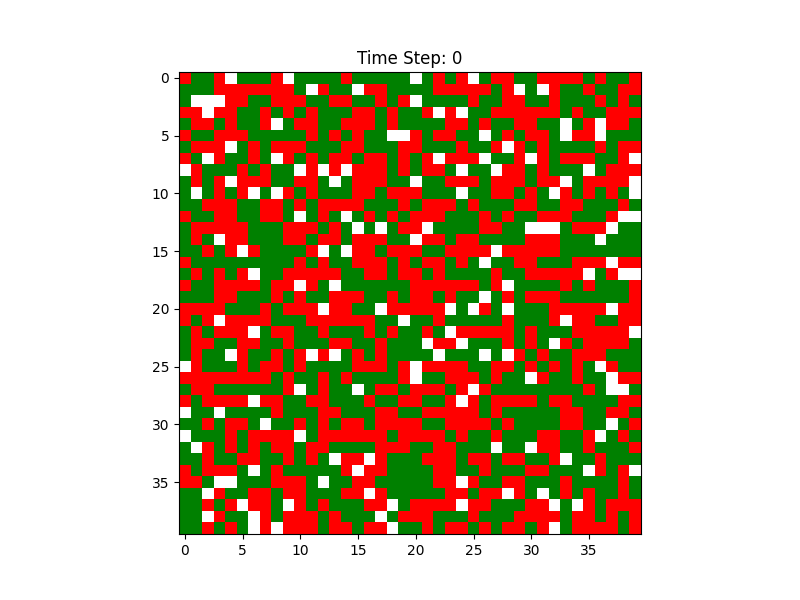
\includegraphics[width=\linewidth]{initial_cluster_w10b10.png}
			\caption{\centering SN w=10, beta=.1}
		\end{subfigure}\hfill
		\begin{subfigure}{0.14\textwidth}
			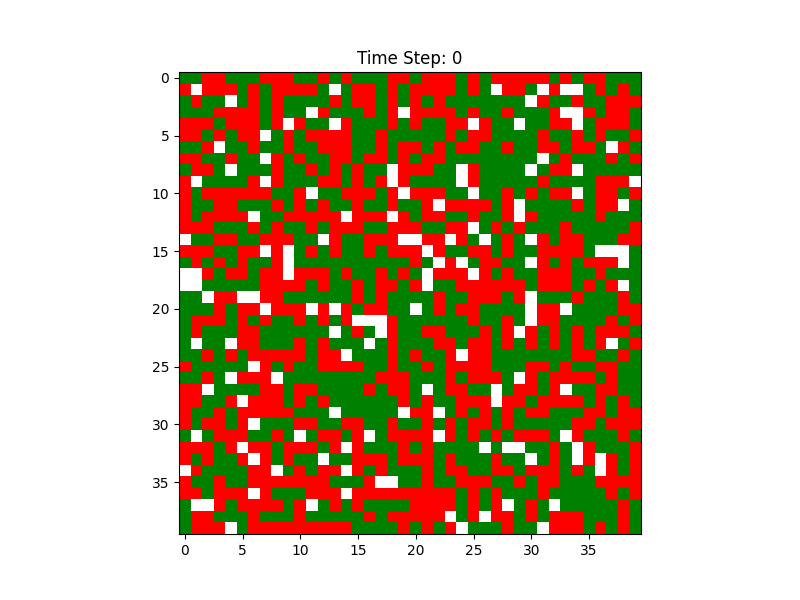
\includegraphics[width=\linewidth]{initial_cluster_w20b10.png}
			\caption{\centering SN w=20, beta=.1}
		\end{subfigure}\hfill
		\begin{subfigure}{0.14\textwidth}
			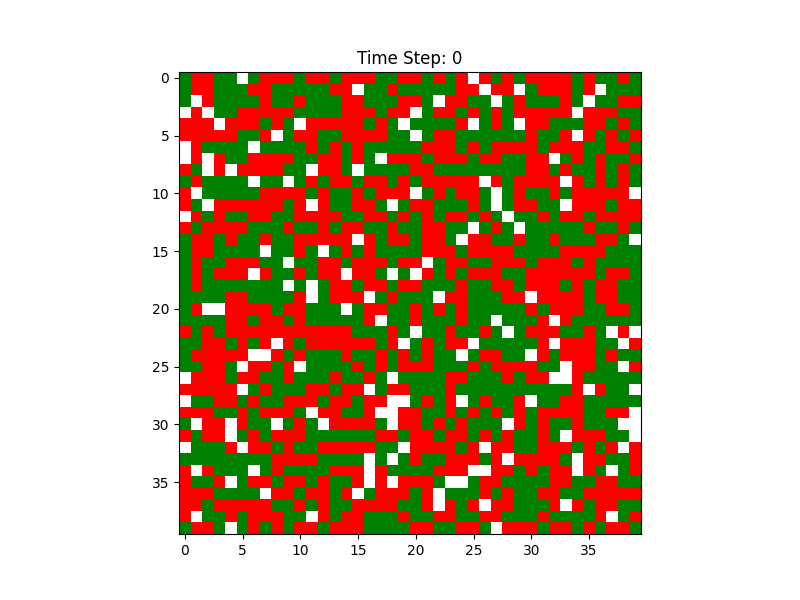
\includegraphics[width=\linewidth]{initial_cluster_w5b20.png}
			\caption{\centering SN w=5, beta=.2}
		\end{subfigure}\hfill
		\begin{subfigure}{0.14\textwidth}
			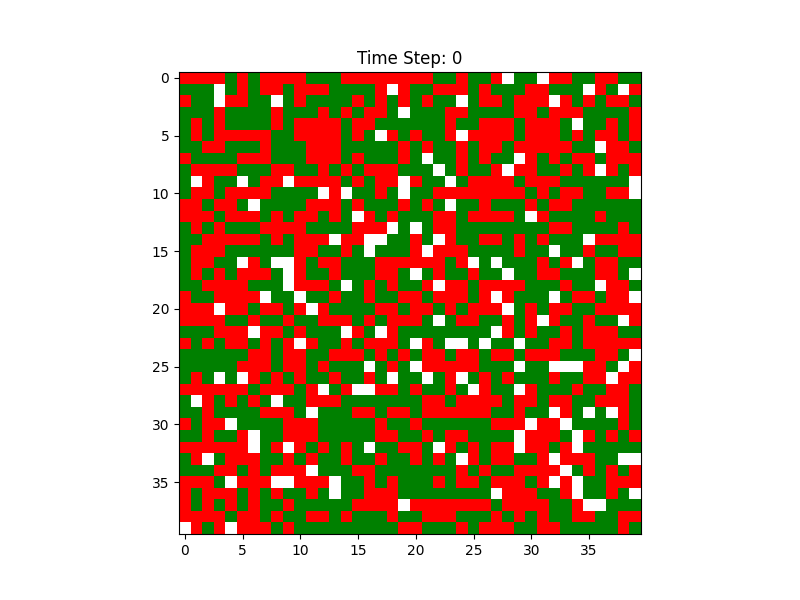
\includegraphics[width=\linewidth]{initial_cluster_w10b20.png}
			\caption{\centering SN w=10, beta=.2}
		\end{subfigure}\hfill
		\begin{subfigure}{0.14\textwidth}
			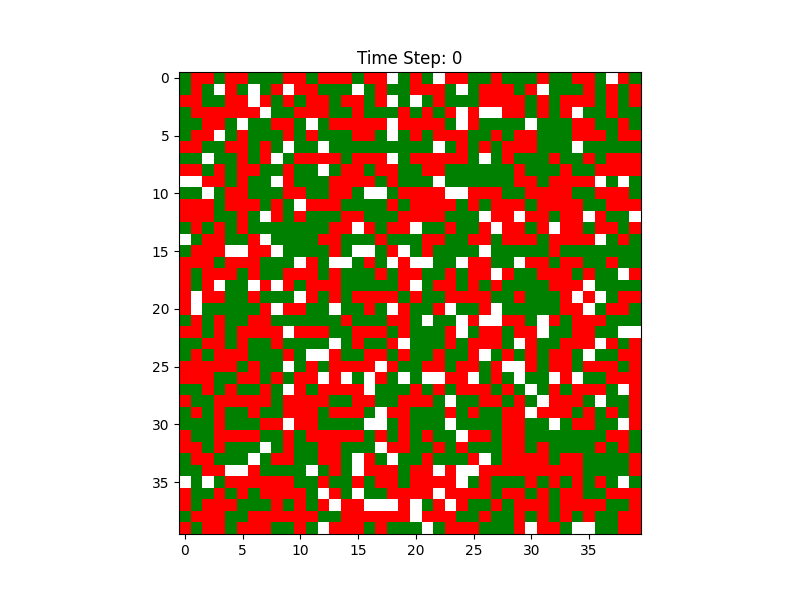
\includegraphics[width=\linewidth]{initial_cluster_w20b20.png}
			\caption{\centering SN w=20, beta=.2}
		\end{subfigure}
		\caption{Initial states of neighborhoods for random move and neighborhood search policy}
	\end{figure}
	\vspace{-2em} % Adjust the vertical space here
	\begin{figure}[h]
		\centering
		\begin{subfigure}{0.14\textwidth}
			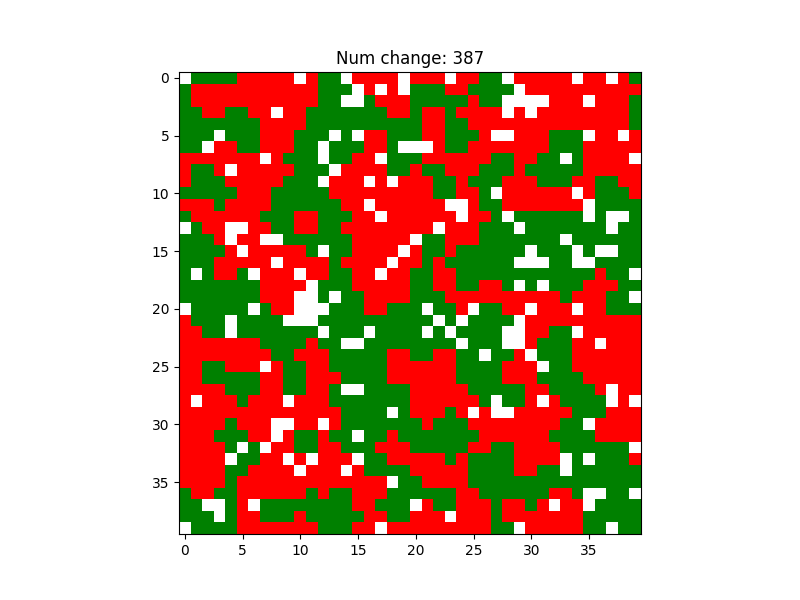
\includegraphics[width=\linewidth]{final_random.png}
			\caption{\centering Random move}
			\label{sn_finalrandom}
		\end{subfigure}\hfill
		\begin{subfigure}{0.14\textwidth}
			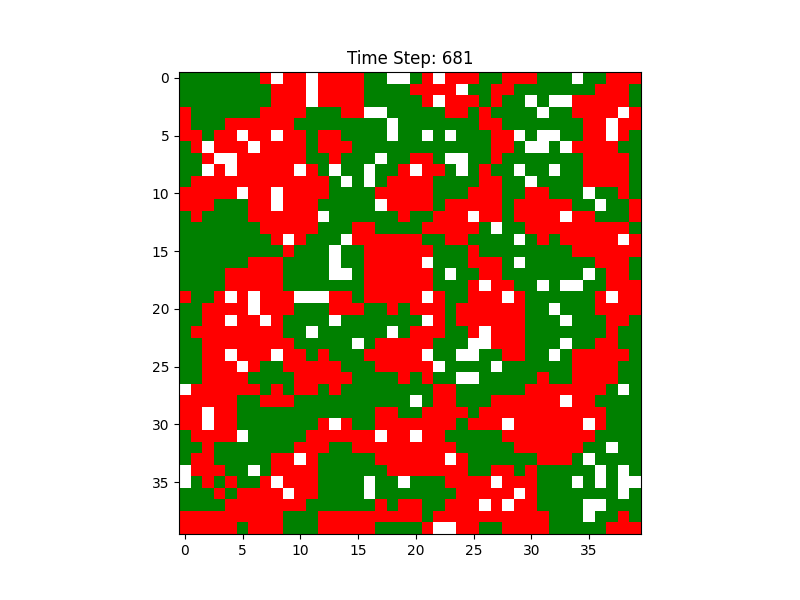
\includegraphics[width=\linewidth]{final_cluster_w5b10.png}
			\caption{\centering SN w=5, beta=.1}
			\label{sn_finalw5b10}
		\end{subfigure}\hfill
		\begin{subfigure}{0.14\textwidth}
			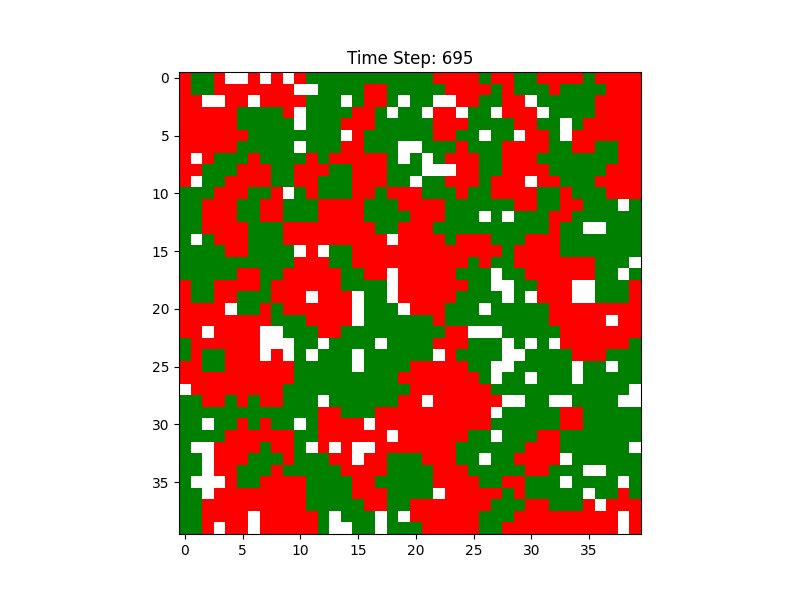
\includegraphics[width=\linewidth]{final_cluster_w10b10.png}
			\caption{\centering SN w=10, beta=.1}
			\label{sn_finalw10b10}
		\end{subfigure}\hfill
		\begin{subfigure}{0.14\textwidth}
			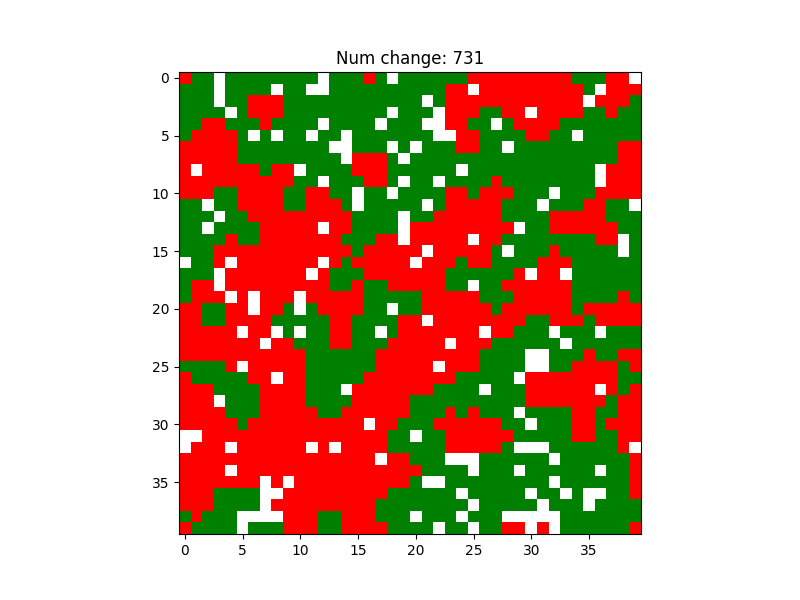
\includegraphics[width=\linewidth]{final_cluster_w20b10.png}
			\caption{\centering SN w=20, beta=.1}
			\label{sn_finalw20b10}
		\end{subfigure}\hfill
		\begin{subfigure}{0.14\textwidth}
			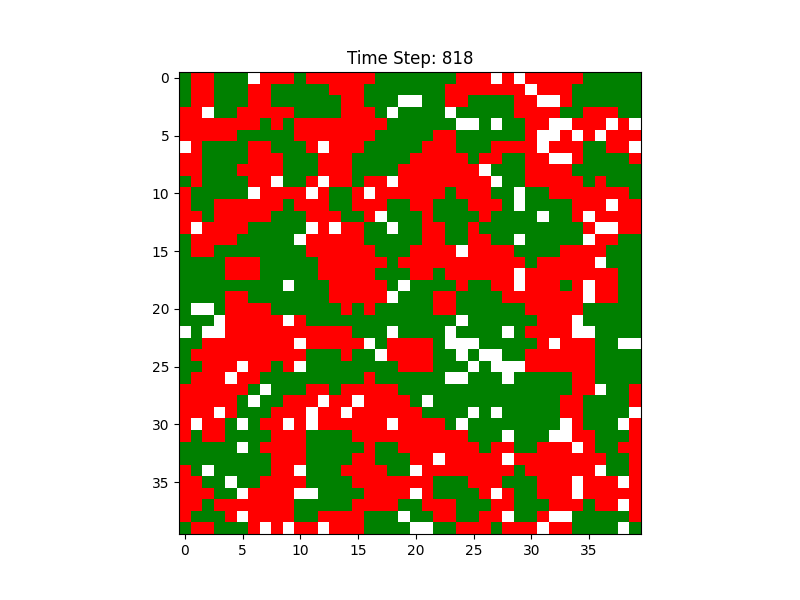
\includegraphics[width=\linewidth]{final_cluster_w5b20.png}
			\caption{\centering SN w=5, beta=.2}
			\label{sn_finalw5b20}
		\end{subfigure}\hfill
		\begin{subfigure}{0.14\textwidth}
			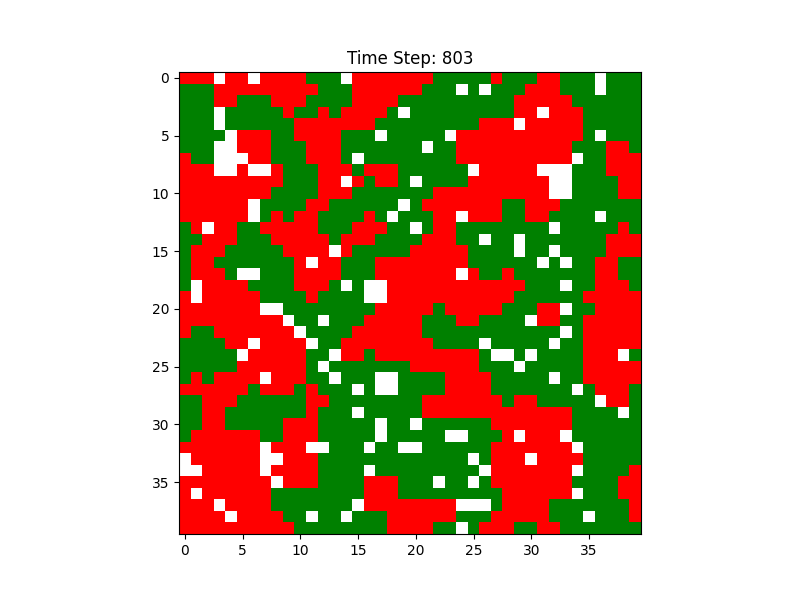
\includegraphics[width=\linewidth]{final_cluster_w10b20.png}
			\caption{\centering SN w=10, beta=.2}
			\label{sn_finalw10b20}
		\end{subfigure}\hfill
		\begin{subfigure}{0.14\textwidth}
			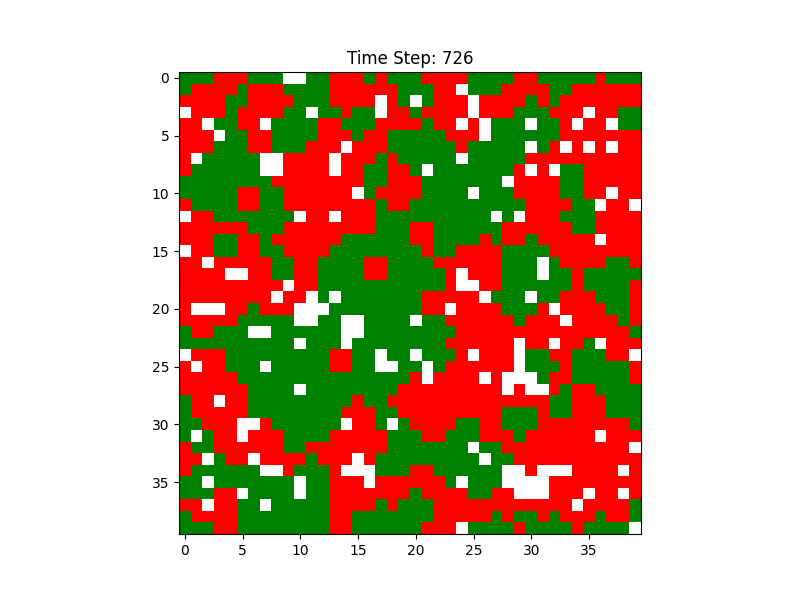
\includegraphics[width=\linewidth]{final_cluster_w20b20.png}
			\caption{\centering SN w=20, beta=.2}
			\label{sn_finalw20b20}
		\end{subfigure}
		\caption{Final states for random move and neighborhood search policies}
		\label{sn_finalstate}
	\end{figure}
	\FloatBarrier
	
	\begin{wrapfigure}{l}{.5\textwidth}
		\centering
		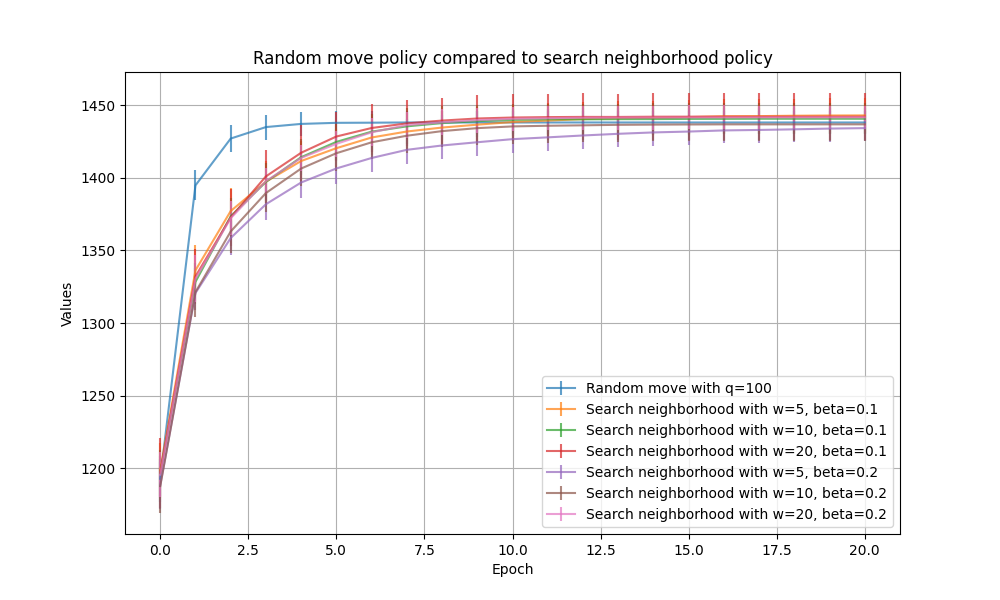
\includegraphics[width=.5\textwidth]{policies02.png}
		\caption{Time series comparison of neighborhood search compared to random move}
	\end{wrapfigure}
	This policy resulted in fully connected clusters across the map of like agents in Fig \ref{sn_finalstate}. The exceptions are small clusters of agents (see Fig \ref{sn_finalw20b20}), which are fully happy while being small enough to not connect to the main cluster. Due to the search only of neighboring spaces, when a cluster of empty spaces appears, it often remains open because its plots are never reported by neighbors; agents also could get stuck until they talk to a mismatched neighbor. This method results in a slower convergence to optimal happiness as the entire automata is not searched but ends up better than the random search as happy neighborhoods form. The neighborhood search with greatest chance of talking to mismatched neighbors in the largest radius was the most successful as it found the most positions. Smaller radii with more matching neighbors asked performed consistently nearly as well though as perhaps makes the agent remain in its own cluster of like agents instead of hopping between  clusters as could occur with a greater $w$. However, the standard deviations are wide enough that an instance of one parameter configuration with lesser average could perform better than another.
	
	\newpage
	
	\subsection{Connor}
	Housing can also be modeled as desireablity to a hotspot; examples being schools, religous buildings, work, etc. To model this, two different hotspots were placed randomly on the grid and red and green agents were set to want to get as close to one of the hotspots as possible. Agents choose from a generated heatmap where the probability of selecting a position is: $e^{\frac{- minimum\ euclidean\ distance\ from\ a\ hotspot}{radius}}$. This formula creates a probability density higher around the center of the arcs. Agents were set to be happy, and therefor not move if they were in a defined closeness value. However, the green agents were able to replace the red agents with the defined probability multipled by one over k. k was varied from 10 to 0.001 in log scale to determine how quickly the green agents could dominate the hotspots. Red agents were unable to replace green agents from their current position.
	
	\subsubsection{Results}
	% for insertion of before/after plots
	\begin{figure}[h]
		\centering
		\begin{subfigure}{0.14\textwidth}
			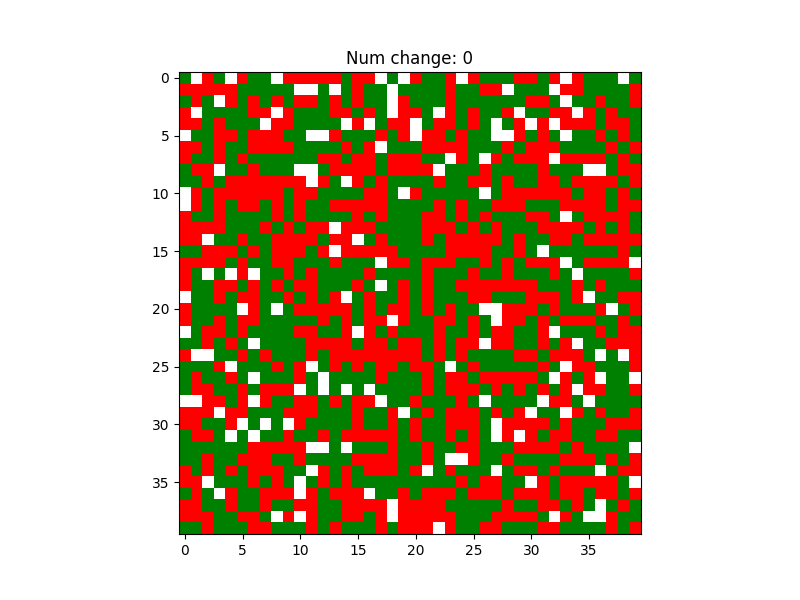
\includegraphics[width=\linewidth]{policy3_initial_h2r5.png}
			\caption{\centering Two Sites with R=5}
		\end{subfigure}\hfill
		\begin{subfigure}{0.14\textwidth}
			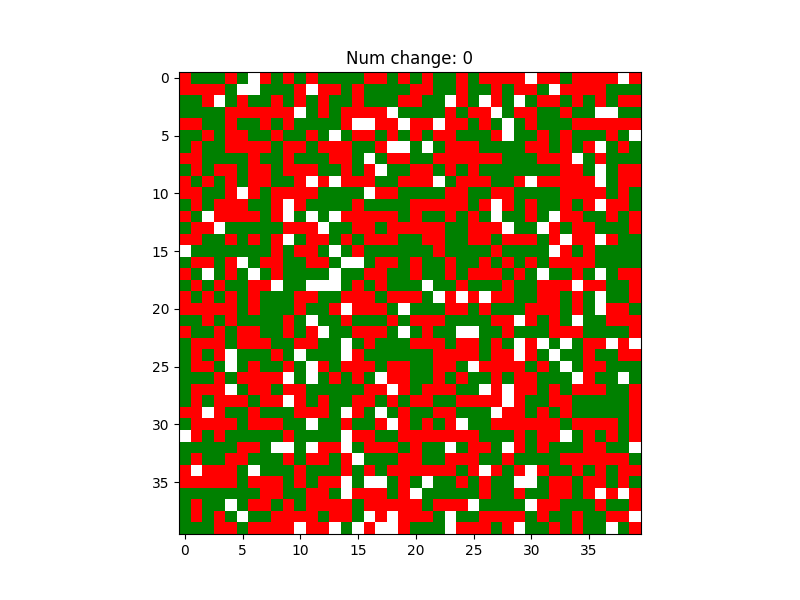
\includegraphics[width=\linewidth]{policy3_initial_h2r10.png}
			\caption{\centering Two Sites with R=10}
		\end{subfigure}\hfill
		\begin{subfigure}{0.14\textwidth}
			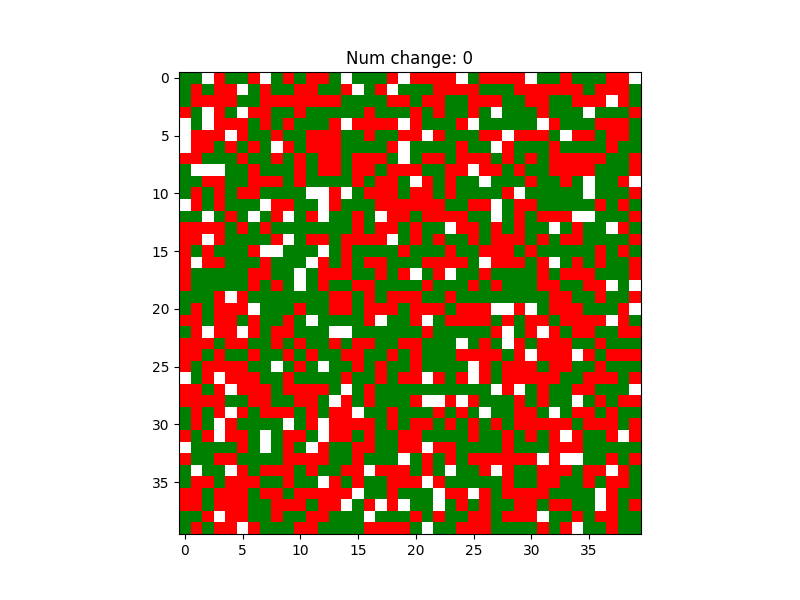
\includegraphics[width=\linewidth]{policy3_initial_h2r15.png}
			\caption{\centering Two Sites with R=15}
		\end{subfigure}\hfill
		\begin{subfigure}{0.14\textwidth}
			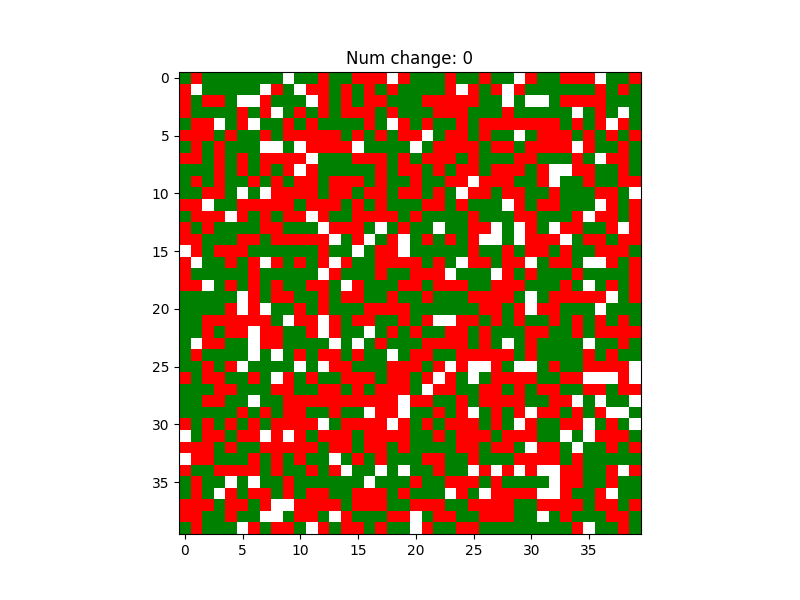
\includegraphics[width=\linewidth]{policy3_initial_h3r5.png}
			\caption{\centering Three Sites with R=5}
		\end{subfigure}\hfill
		\begin{subfigure}{0.14\textwidth}
			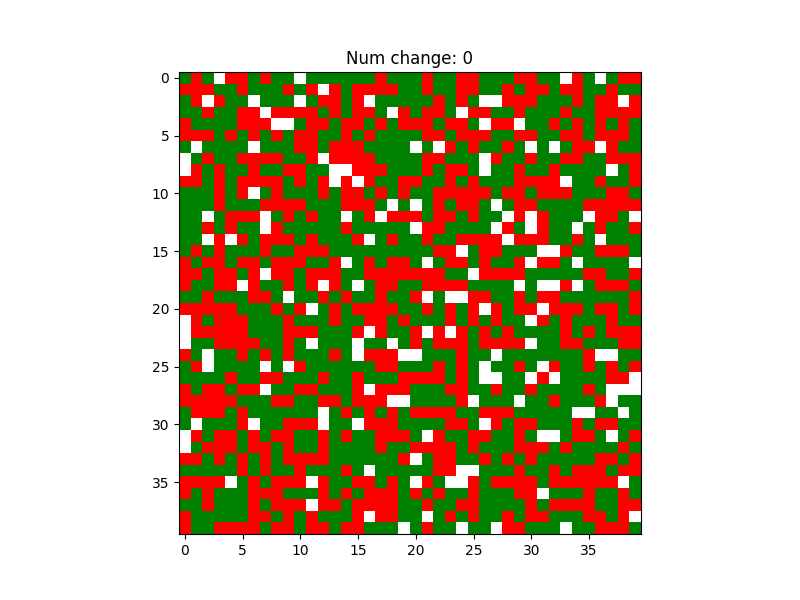
\includegraphics[width=\linewidth]{policy3_initial_h3r10.png}
			\caption{\centering Three Sites with R=10}
		\end{subfigure}\hfill
		\begin{subfigure}{0.14\textwidth}
			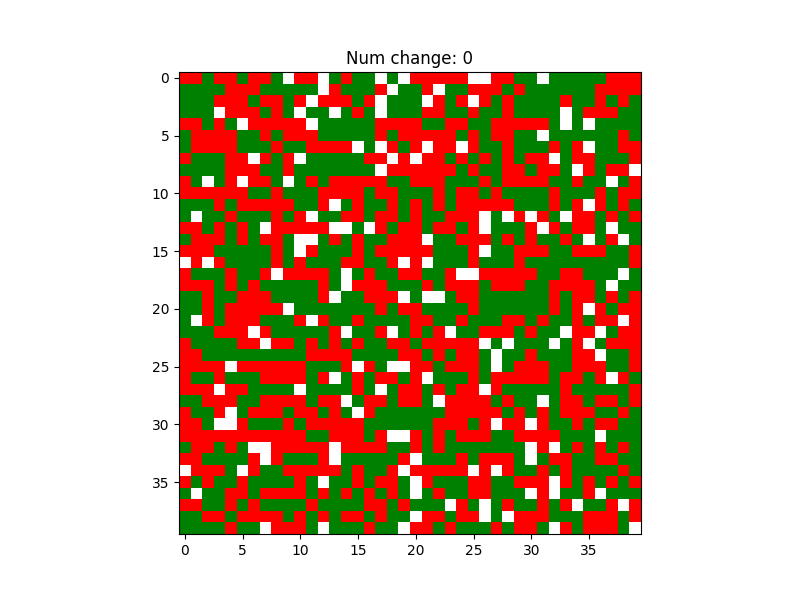
\includegraphics[width=\linewidth]{policy3_initial_h3r15.png}
			\caption{\centering Three Sites with R=15}
		\end{subfigure}\hfill
		\caption{Initial States of Neighborhoods for Site Relocation Policy}
	\end{figure}
	\vspace{-2em} % Adjust the vertical space here
	\begin{figure}[h]
		\centering
		\begin{subfigure}{0.14\textwidth}
			\includegraphics[width=\linewidth]{policy3_Final_h2r5.png}
			\caption{\centering Two Sites with R=5}
		\end{subfigure}\hfill
		\begin{subfigure}{0.14\textwidth}
			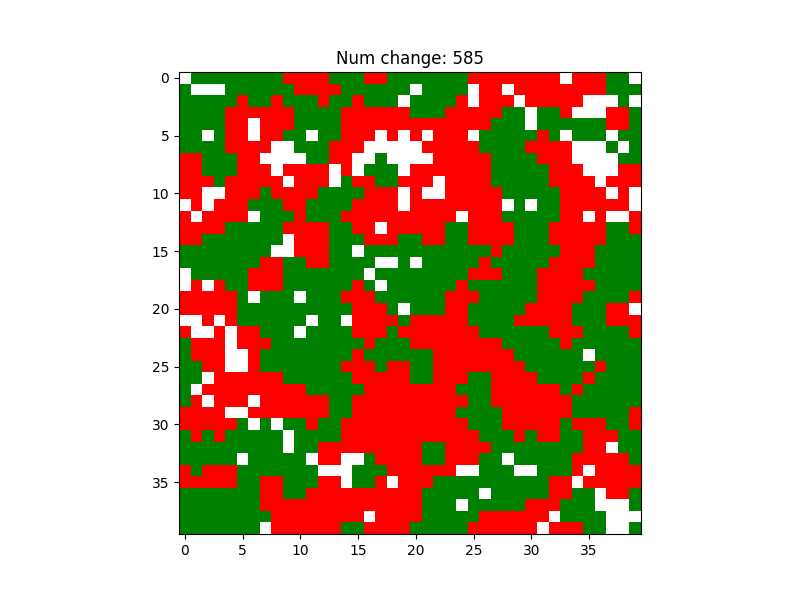
\includegraphics[width=\linewidth]{policy3_final_h2r10.png}
			\caption{\centering Two Sites with R=10}
		\end{subfigure}\hfill
		\begin{subfigure}{0.14\textwidth}
			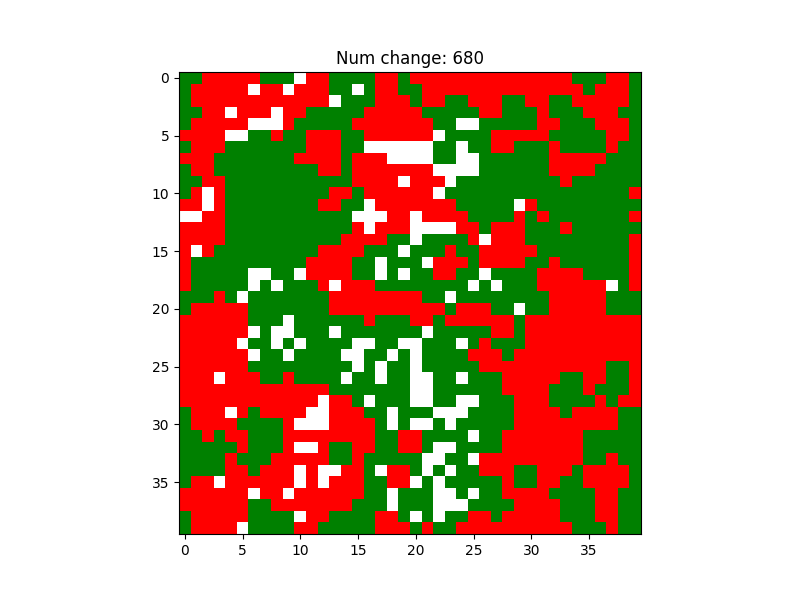
\includegraphics[width=\linewidth]{policy3_final_h2r15.png}
			\caption{\centering Two Sites with R=15}
		\end{subfigure}\hfill
		\begin{subfigure}{0.14\textwidth}
			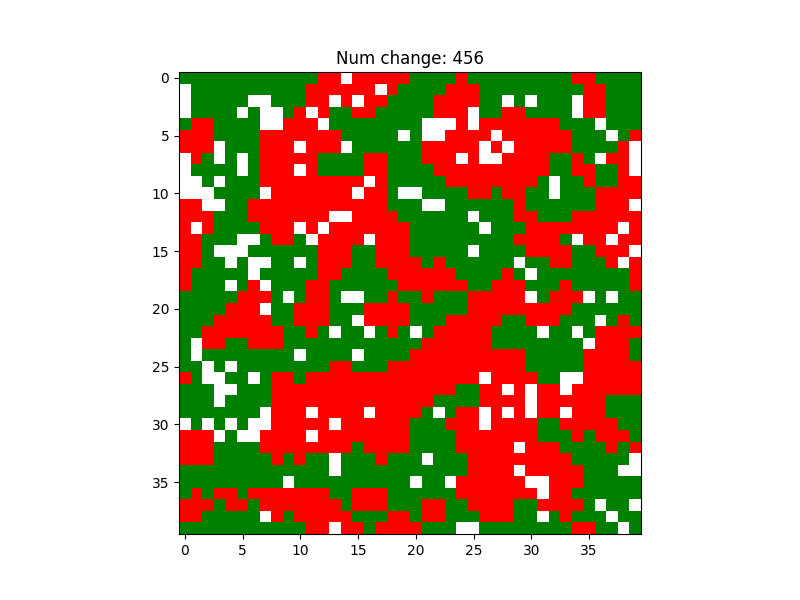
\includegraphics[width=\linewidth]{policy3_final_h3r5.png}
			\caption{\centering Three Sites with R=5}
		\end{subfigure}\hfill
		\begin{subfigure}{0.14\textwidth}
			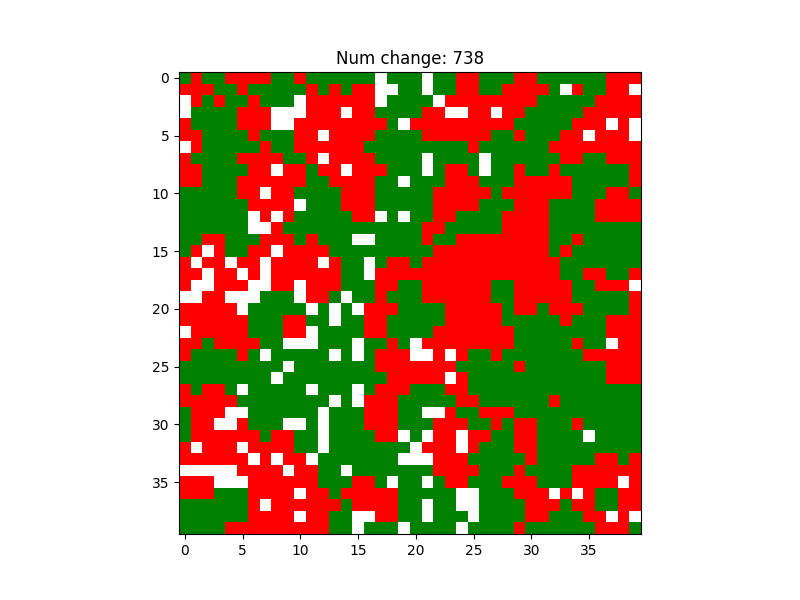
\includegraphics[width=\linewidth]{policy3_final_h3r10.png}
			\caption{\centering Three Sites with R=10}
		\end{subfigure}\hfill
		\begin{subfigure}{0.14\textwidth}
			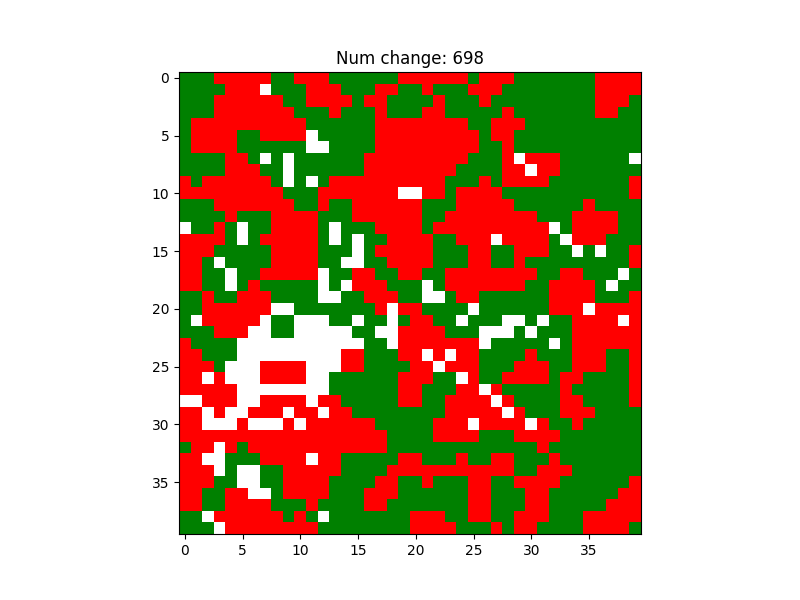
\includegraphics[width=\linewidth]{policy3_final_h3r15.png}
			\caption{\centering Three Sites with R=15}
		\end{subfigure}
		\caption{Final States of Neighborhoods for Site Relocation Policy}
	\end{figure}
	\FloatBarrier
	
	\begin{wrapfigure}{l}{.5\textwidth}
		\centering
		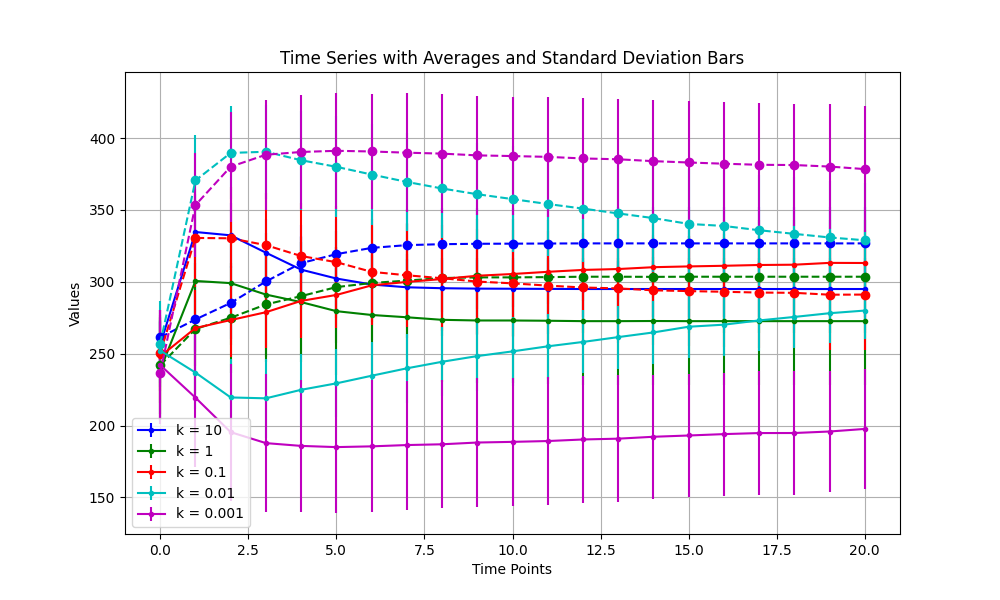
\includegraphics[width=.5\textwidth]{policies03.png}
		\caption{Time series comparing Random Move to Site Relocation Policy by Varying both Amount and Radii of Hotspots}
		\label{p3_ts}
	\end{wrapfigure}
	\FloatBarrier
	Initially, Fig both the red and green agents were able to coexist near the hotspots. However, as shown in Fig \ref{p3_final_0001}, the green agents eventually dominate and take up most of the area's around the hotspots. This is also clear in Fig \ref{p3_ts} where for k = 10 to 0.01, both the agent groups on average were happier after they were allowed to move. However, as k decreased to 0.001, a large transition happened were the red agents become significantly unhappier than in their starting states. This model can help demonstate the adventages of giving a group the power to evict another group and the eventual domination of a resource of that group. It is interesting that it did require a significant drive, on the scale of 1000 times their inital probability, for the green agents to entirely dominate. Different variations could be performed such as agumenting the probability equaiton so that the most desireable locations are those that are closest to both of the hotspots, varying the radius of the hotspot, or varying the agents happiness with their closeness. 
	
	
	\newpage
	
	\subsection{Josh}
	
	


	
\end{document}